\section{凝聚态系统的构成}

普通的固体、液体、气体由一系列原子组成。通过实验和计算可以发现,原子的最外层电子在各种过程中容易发生重新排列,称为\concept{价电子};内层电子和原子核(合称为\concept{离子实})则通常保持为一个整体,也即,其内部状态发生变化的物理过程的描述需要使用QCD,其涉及的能标远高于价电子发生变化涉及的能标。

本文基本上只分析涉及价电子低能运动的物理过程,即只讨论非相对论极限下的电荷-电磁场耦合系统,而忽略强相互作用、弱相互作用和引力。
此时,带电粒子由薛定谔场完全描述,系统具有$U(1)$规范对称性且无粒子数生灭,有确定的粒子数,于是可以原则上实物粒子部分可以直接用单粒子量子力学描述。
进一步,我们假定系统中没有变化特别快的电磁场,这意味着实际上我们可以积掉电磁场并且得到一个延迟不明显的相互作用,那就是说,我们可以把所有电磁相互作用都用静电学和静磁学处理。由于无论是电子还是离子实都是非相对论性的,电子-电子相互作用、电子-离子实相互作用、离子实-离子实相互作用几乎完全是库伦相互作用。

\subsection{电子}

\subsubsection{电子动能和库伦排斥能}

设有$N_e$个价电子,$N_i$个离子实(i表示离子),固体的不考虑外界扰动的一次量子化哈密顿量为
\begin{equation}
    {H} = {H}_\text{e} + {H}_\text{i} + {H}_\text{ei},
    \label{eq:many-body-hamiltonian}
\end{equation}
其中${H}_\text{e}$表示仅涉及价电子的哈密顿量,${H}_\text{i}$表示仅涉及离子实的哈密顿量,最后一项则是两者的相互作用,所有相互作用是库仑相互作用。
诸价电子组成的系统就好像由电子组成的气体,称为\concept{相互作用电子气}。单体哈密顿量为电子的动能项加上单体势能项。在物质不受外界作用时当然不应该有单体势能项,于是
\[
    {H}_\text{e1} = \frac{{\vb*{p}}^2}{2m},
\]
在坐标表象下它就是
\[
    {H}_\text{e1} = - \frac{\laplacian}{2m}.
\]
二体哈密顿量为电子两两作用而产生的库伦势能是
\[
    {H}_\text{e2} = \frac{e^2}{\abs{\vb*{r}_1 - \vb*{r}_2}},
\]
从而价电子本身的能量以及它们之间发生库伦相互作用的能量就是
\begin{equation}
    {H}_\text{e} = \sum_{i=1}^{N_\text{e}} \frac{{p}_i^2}{2m_\text{e}} + \frac{1}{2} \sum_{i\neq j} \frac{e^2}{\abs{\vb*{r}_i - \vb*{r}_j}}.
\end{equation}
使用类似的方法,离子实的组成的系统(如果是晶体那就是晶格)的哈密顿量为
\begin{equation}
    {H}_\text{i} = \sum_{\alpha=1}^{N_\text{i}} \frac{{p}_\alpha^2}{2m_i} + \frac{1}{2} \sum_{\alpha\neq\beta} V(\vb*{R}_\alpha-\vb*{R}_\beta).
\end{equation}
由于离子实中的内层电子结构复杂,离子实之间的相互作用能写不出特别简单的表达式(我们相当于把内层电子的自由度也积掉了)。请注意这个相互作用能是平移不变的,这是当然的,因为QED是平移不变的;但是实际的固体在短距离上并不是平移不变的,因为在低能下有对称性自发破缺。
离子实和价电子的相互作用则是
\begin{equation}
    {H}_\text{ei} = \sum_{\alpha, i} V_\text{ei}(\vb*{r}_i-\vb*{R}_\alpha). 
\end{equation}
分别使用$i$表示价电子,用$\alpha$表示离子实;由于价电子和离子实不全同,不需要加上$1/2$系数。
同样我们还是假定了相互作用本身的平移不变性。
本文仅仅讨论固体(实际上主要是晶体)的物理,因此我们将假定离子实的位移始终局限在非常小的范围内。

在大部分过程中,由于原子核的质量比电子的质量大至少三个数量级,涉及价电子的过程通常比涉及离子实的过程发生得快很多,从而在价电子的时间尺度上,诸离子实的位置可以看成是给定的。
从而,在分析价电子时我们可以将${H}_i$项直接略去,而将${H}_\text{ei}(\vb*{r}_i-\vb*{R}_\alpha)$项对$\vb*{R}_\alpha$求和得到$V_\text{ext}(\vb*{r}_i)$(使用ext为下标是因为离子实相当于是给相互作用电子气施加了一个外场)。这个近似称为\concept{玻恩–奥本海默近似}。这样一来相互作用电子气的一次量子化哈密顿量在坐标表象下就是
\begin{equation}
    {H} = \sum_{i=1}^{N_\text{e}} \left( - \frac{\laplacian}{2m_\text{e}} + V_\text{ext}(\vb*{r}_i)\right) + \frac{1}{2} \sum_{i\neq j} \frac{e^2}{\abs{\vb*{r}_i - \vb*{r}_j}},
    \label{eq:electron-gas-hamiltonian}
\end{equation}
从而二次量子化哈密顿量为
\begin{equation}
    \begin{aligned}
        {H} = &\sum_{\sigma} \int \dd[3]{\vb*{r}} {\psi}_\sigma^\dagger(\vb*{r}) \left( - \frac{\laplacian}{2m} + V_\text{ext}(\vb*{r}) \right) {\psi}_\sigma(\vb*{r}) \\
        &+ \frac{1}{2} \sum_{\alpha, \beta} \int \dd[3]{\vb*{r}_1} \int \dd[3]{\vb*{r}_2} 
        {\psi}_\alpha^\dagger (\vb*{r}_1) {\psi}_\beta^\dagger (\vb*{r}_2) \frac{e^2}{\abs{\vb*{r}_1 - \vb*{r}_2}} {\psi}_\beta (\vb*{r}_2) {\psi}_\alpha (\vb*{r}_1). 
    \end{aligned}
    \label{eq:electron-gas-hamiltonian-sq}
\end{equation}
其中${\psi}^\dagger(\vb*{r})$是薛定谔场的场算符,它也是在位置为$\vb*{r}$的位置产生一个电子的产生算符。这个哈密顿量当然也可以通过QED的低能近似得到,但并没有必要这么做。请注意电子是费米子。
\eqref{eq:electron-gas-hamiltonian-sq}实际上不是对角的,因为它的单粒子项涉及一个梯度算符。

需要注意的是实际上仍然可能有电子和离子实的相互作用(即电子-声子相互作用),因此波恩-奥本海默近似中的电子质量和电子-电子相互作用的具体形式可能出现和该相互作用相关的跑动,此时\eqref{eq:electron-gas-hamiltonian-sq}中的所谓“电子”已经是一种准粒子了。

最后我们指出,由于固体始终可以和外界交换电子——外界的电子可以进入固体,固体中的电子可以溢出——固体中电子气本身的哈密顿量\eqref{eq:electron-gas-hamiltonian-sq}不足以充分描述系统。
本文将只研究近平衡系统,因此这种与外界的相互作用可以使用化学势描述,即我们需要在\eqref{eq:electron-gas-hamiltonian-sq}中加入一项$-\mu {\psi}^\dagger(\vb*{r}) {\psi}(\vb*{r})$,这样得到的哈密顿量才是完整的。
换而言之,电子气完整的哈密顿量形如
\begin{equation}
    \begin{aligned}
        {H} &= \sum_{\vb*{k}, \sigma} \Big( \underbrace{\frac{\vb*{k}^2}{2m}}_{\epsilon_{\vb*{k}}} - \mu \Big) {c}^\dagger_{\vb*{k} \sigma} {c}_{\vb*{k} \sigma} 
        + \int \dd[3]{\vb*{r}} V_\text{ext}(\vb*{r}) {\psi}^\dagger(\vb*{r}) {\psi}(\vb*{r}) \\ 
        &+ \frac{1}{2} \sum_{\alpha, \beta} \int \dd[3]{\vb*{r}_1} \int \dd[3]{\vb*{r}_2} 
        {\psi}_\alpha^\dagger (\vb*{r}_1) {\psi}_\beta^\dagger (\vb*{r}_2) \frac{e^2}{\abs{\vb*{r}_1 - \vb*{r}_2}} {\psi}_\beta (\vb*{r}_2) {\psi}_\alpha (\vb*{r}_1).
    \end{aligned}
    \label{eq:full-electron-gas-hamiltonian}
\end{equation}
在有些模型中有时也将外势场并入$\epsilon_{\vb*{k}}$项。
为了简便起见,通常用$\xi$表示扣除了化学势的单电子能量,即
\begin{equation}
    \xi_{\vb*{k}} = \epsilon_{\vb*{k}} - \mu.
\end{equation}

\subsubsection{哈密顿量的一般形式}

以上我们都是将库伦相互作用加入薛定谔场中,可以说是给出了第一性原理计算需要的哈密顿量(虽然实际上从高能物理的角度这远非第一性原理,但对凝聚态理论来说通常已经够用了)。
但实际上还有以下机制没有考虑:
\begin{itemize}
    \item 作用在单体上的外场的束缚,离子实的束缚已经被计入考虑了,但是还有其它外场,比如说或许会有一个磁场,然后哈密顿量中将会有一项$-\vb*{\mu} \cdot \vb*{B}$;无论如何这会是一个二体算符。
    \item 电子-声子相互作用会引入一个二电子和一个声子发生相互作用的顶角,积掉声子自由度之后会留下一个等效的电子-电子相互作用,这会让\eqref{eq:full-electron-gas-hamiltonian}中电子-电子相互作用的系数发生变化,不再是严格的库伦排斥。
\end{itemize}
于是我们写出一般形式的相互作用电子气的二次量子化哈密顿量:
\begin{equation}
    {H} = \sum_{\vb*{k}, \sigma} (T_{\vb*{k}} - \mu) {c}^\dagger_{\vb*{k} \sigma} {c}_{\vb*{k} \sigma} 
    + \sum_{\vb*{k}_1, \vb*{k}_2, \sigma} V^\text{ext}_{\vb*{k}_1 \vb*{k}_2 \sigma} {c}^\dagger_{\vb*{k}_1 \sigma} {c}_{\vb*{k}_2 \sigma}
    + \sum_{\vb*{k}_1, \vb*{k}_2, \vb*{q}, \alpha, \beta} {c}^\dagger_{\vb*{k}_1+\vb*{q}, \alpha} {c}^\dagger_{\vb*{k}_2-\vb*{q}, \beta} V_{\vb*{q}} {c}_{\vb*{k}_2 \beta} {c}_{\vb*{k}_1 \alpha}. 
\end{equation}
相应的,热力学作用量为
\begin{equation}
    S = \sum_n \left( 
        \sum_{\vb*{k}, \sigma} (-\ii \omega_n + T_{\vb*{k}} - \mu) \bar{c}_{\vb*{k} \sigma} c_{\vb*{k} \sigma} 
        + \sum_{\vb*{k}_1, \vb*{k}_2, \sigma} V^\text{ext}_{\vb*{k}_1 \vb*{k}_2 \sigma} \bar{c}_{\vb*{k}_1 \sigma} c_{\vb*{k}_2 \sigma} 
        + \sum_{\vb*{k}_1, \vb*{k}_2, \vb*{q}, \sigma} \bar{c}_{\vb*{k}_1+\vb*{q}, \sigma} \bar{c}_{\vb*{k}_2-\vb*{q}, \sigma} V_{\vb*{q}} c_{\vb*{k}_2 \sigma} c_{\vb*{k}_1 \sigma} \right). 
\end{equation}
上式中的动能项和相互作用项的形式由对称性确定,具体系数可以暂时不设置具体值(因为直接从\eqref{eq:full-electron-gas-hamiltonian}出发做重整化群计算显然是非常困难的)。
处理这类模型的常用方法包括:
\begin{itemize}
    \item 直接做费曼图计算(需要注意由于库伦相互作用是瞬时的,通常将库仑相互作用顶角写成用虚线连接的两个顶角,每个顶角有一个电子入射和一个电子出射,虚线可以携带动量),由于相互作用是二体的,在相互作用较弱时计算一到二圈图就可以得到很好的效果,不过实际上相互作用并不总是那么弱,此时需要一些其它近似手段;
    \item 由于相互作用项是四阶的,可以使用Hubbard-Stratonovich变换引入一个辅助场,通过适当选取辅助场(通常要和某个有趣的序参量具有同样的对称性)并积掉电子自由度,则接近临界点时,辅助场满足的场论就给出了长程自由度;
    \item 做平均场计算并与实验或数值计算作比较(可以对原来的模型做平均场也可以对Hubbard-Stratonovich变换之后的辅助场做平均场);
    \item 在定性论证出来一些现象后考虑其上的涨落,获得一个关于平均值附近涨落的理论(可以和平均场一起使用);
    \item 近似处理,如忽略一部分动能(即忽略一部分电子跃迁项),或者简化相互作用形式。
\end{itemize}
无论如何,凝聚态模型通常都足够复杂,且可能有很强的相互作用,以至于分析方法多种多样,但是没有哪一种能够占有支配地位。

\subsubsection{外加电磁场}

现在讨论外加电磁场导致的哈密顿量变化,或者说“辐射和物质相互作用”导致的哈密顿量变化。
一般的,设系统被放置在电磁场$(\varphi, \vb*{A})$中,则一次量子化哈密顿量(使用一次量子化哈密顿量是为了和经典的“一群电子定向移动”的物理图像对应上)为
\begin{equation}
    {H} = \frac{1}{2m} \sum_i ({\vb*{p}_i} - q_i \vb*{A}({\vb*{r}_i}))^2 + \sum_i q_i \varphi({\vb*{r}}_i) + {H}_\text{int},
    \label{eq:hamiltonian-with-eb-original}
\end{equation}
其中$\vb*{p}$是正则动量,${H}_\text{int}$表示粒子间相互作用。
本文仅考虑外加电磁场产生的线性响应,于是考虑辐射场不很强以至于$\vb*{A}^2$可以忽略的情况,也即,仅保留单光子过程,忽略一切$\vb*{A}^2$项。
% TODO:真的吗?实际上,当辐射场强到非线性效应开始产生时,是不是应该单独列出来一个${H}_\text{int}$然后将物质和辐射做$U(1)$极小耦合已经很成问题了:
在\eqref{eq:hamiltonian-with-eb-original}中我们将电子间的库伦排斥能和辐射场引入的能量简单相加,因为这的确是两种不同的过程:库伦排斥涉及的光子实际上是不满足横场条件的虚光子,而辐射场中的光子都是可以出现在实际的物理态中的光子。

对电子系统,$q=-e$,那么就有
\begin{equation}
    \begin{aligned}
        {H} &= \frac{1}{2m} \sum_i ({\vb*{p}_i} + e \vb*{A}({\vb*{r}_i}))^2 - e \sum_i \varphi({\vb*{r}}_i) + {H}_\text{int} \\ 
        &= - \frac{1}{2m} \sum_i (\grad + \ii e \vb*{A}({\vb*{r}_i}))^2 - e \sum_i \varphi({\vb*{r}}_i) + {H}_\text{int}.
    \end{aligned}
\end{equation}
设$\Omega$是某个空间区域,电流密度为$\vb*{J}$,则
\begin{equation}
    \int_\Omega \dd[3]{\vb*{r}} {\vb*{J}} = - \sum_i e {\vb*{v}}_i,
\end{equation}
其中$\vb*{v}_i$是电子移动的速度,满足
\begin{equation}
    {\vb*{v}}_i = \pdv{H}{\vb*{r}_i} = \frac{{\vb*{p}}_i + e \vb*{A}({\vb*{r}}_i)}{m}.
\end{equation}
考虑到$\Omega$的任意性,我们就有以下近似表达式:
\begin{equation}
    {\vb*{J}} = \underbrace{- \frac{e}{m} \sum_i ( \delta(\vb*{r} - {\vb*{r}}_i) {\vb*{p}} + {\vb*{p}} \delta(\vb*{r} - {\vb*{r}}_i) )}_{{\vb*{j}}} \underbrace{- \frac{e^2}{m} {n}_\text{e}}_{{\vb*{j}}_\text{D}} \vb*{A}.
\end{equation}
${\vb*{j}}$项特意被写成了厄米的形式;${\vb*{j}}_\text{D}$已经做了一遍粗粒化了,将诸$\vb*{A}_i$平均了一遍。
通常这是合理的,因为电磁波的波长通常不会特别小,从而不会有很大的空间起伏。(而如果有很大的空间起伏,我们就会使用cQED而不是经典电动力学讨论问题了)

现在写出略去高阶项的哈密顿量的形式。选取库伦规范,并认为$\varphi=0$,此时会发现,实际上我们有
\[
    {H} = \frac{1}{2m} \sum_i {\vb*{p}}_i^2 + {H}_\text{int} + \frac{e}{m} \sum_i {\vb*{p}}_i \cdot \vb*{A}({\vb*{r}}_i) - e \sum_i \varphi({\vb*{r}_i}),
\]
$\vb*{A}({\vb*{r}}_i)$和${\vb*{p}}_i$本来是不对易的,但是库伦规范下它们对易。
代入${\vb*{J}}$的表达式并再次略去高阶项,就有
\[
    {H} = \frac{1}{2m} \sum_i {\vb*{p}}_i^2 + {H}_\text{int} - \int \dd[3]{\vb*{r}} {\vb*{J}} \cdot \vb*{A} - e \sum_i \varphi({\vb*{r}_i}).
\]
至于含有电势的那一项,注意到电荷密度为
\[
    {\rho} = - e \sum_{i} \delta({\vb*{r}}_i - \vb*{r}),
\]
于是最后得到
\begin{equation}
    {H} = \frac{1}{2m} \sum_i {\vb*{p}}_i^2 + {H}_\text{int} + \int \dd[3]{\vb*{r}} \varphi {\rho} - \int \dd[3]{\vb*{r}} {\vb*{J}} \cdot \vb*{A}.
\end{equation}
虽然物质本身的哈密顿量不是洛伦兹协变的(因为取了非相对论近似),但是物质和辐射的相互作用项却是洛伦兹协变的——对电磁场的描述一般都是如此。
以上哈密顿量实际上仅仅讨论了轨道部分,电子还有自旋磁矩
\[
    {H}_{\text{spin}} = \sum_i {\vb*{\mu}}_i \cdot \vb*{B}({\vb*{r}}_i),
\]
我们可以如法炮制地将它写成
\[
    {H}_{\text{spin}} = \int \dd[3]{\vb*{r}} {\vb*{\mu}} \cdot \vb*{B}.
\]
因此完整的哈密顿量实际上是
\begin{equation}
    {H} = - \frac{1}{2m} \sum_i {\vb*{p}}_i^2 + {H}_\text{int} + \int \dd[3]{\vb*{r}} \varphi {\rho} - \int \dd[3]{\vb*{r}} {\vb*{J}} \cdot \vb*{A} + \int \dd[3]{\vb*{r}} {\vb*{\mu}} \cdot \vb*{B}.
    \label{eq:hamiltonian-with-eb}
\end{equation}
所有和单粒子携带的电荷数量有关的量全部被藏在电荷密度和电流密度中了,上式在电荷正反变换下不变。

\eqref{eq:hamiltonian-with-eb}当然也可以非常容易地写成二次量子化的形式。
薛定谔场满足$U(1)$对称性,因此通过诺特定理可以得到守恒荷(当然就是电荷)
\begin{equation}
    \rho = - e \sum_\sigma {\psi}^\dagger_\sigma {\psi}_\sigma = - e {n}_\text{e},
\end{equation}
守恒流(也即电流密度)
\begin{equation}
    {\vb*{j}} = - \frac{\ii e}{2m} \sum_\sigma ({\psi}_\sigma^\dagger(\vb*{r}) \grad{{\psi}_\sigma}(\vb*{r}) - (\grad{{\psi}_\sigma^\dagger}(\vb*{r})) {\psi}_\sigma(\vb*{r})) - \frac{e^2}{m} \vb*{A}(\vb*{r}) \sum_\sigma {\psi}^\dagger_\sigma(\vb*{r}) {\psi}_\sigma(\vb*{r}),
\end{equation}
而另一方面自旋磁矩为
\begin{equation}
    {\vb*{\mu}} = {\psi}^\dagger_\alpha \vb*{\sigma}_{\alpha \beta} {\psi}_\beta.
\end{equation}
这样就把三个对外加电磁场的线性响应全部写成二次量子化的形式了;我们可以用推迟格林函数计算出有关的响应大小。

由线性响应理论,我们有
\[
    \begin{aligned}
        \expval*{{J}_i}_A (t) &= \expval*{{J}_i}_0 + \ii \int \dd{t} \int \dd[3]{\vb*{r}'} \theta(t-t') \expval*{\comm*{{J}_i(\vb*{r}, t)}{{J}_j(\vb*{r}', t')}} A_j(\vb*{r}', t') \\
        &= - \frac{e^2}{m} \expval*{{n}_\text{e}} A_i + \ii \int \dd{t} \int \dd[3]{\vb*{r}'} \theta(t-t') \expval*{\comm*{{j}_i(\vb*{r}, t)}{{j}_j(\vb*{r}', t')}} A_j(\vb*{r}', t').
    \end{aligned}
\]
这里的$i, j$为维度脚标,并不表示粒子编号,且使用爱因斯坦求和约定;下标$A$表示有外场$\vb*{A}$时的期望值;${j}_i$的无外场期望是零,这是对称性的结果。

实际上,电阻率定义为%
\footnote{$\vb*{A}(\vb*{r}, t)$完全可以不是时间、空间平移不变的,但是既然我们将$\vb*{A}$当成扰动,只需要无扰动的系统的动力学时间、空间平移不变即可。}%
\begin{equation}
    J_i(\vb*{r}, t) = \int \dd[3]{\vb*{r}'} \int_{-\infty}^t \sigma_{ij}(\vb*{r}-\vb*{r}', t - t') E_j(\vb*{r}', t'),
\end{equation}
于是为了避免繁琐的时间上的微积分我们切换到频域上,有
% TODO:确认记号问题

现在我们回到二次量子化的框架下,考虑怎么计算有关的推迟格林函数。

在虚时间路径积分中不能简单地将\eqref{eq:hamiltonian-with-eb-original}(从而,\eqref{eq:hamiltonian-with-eb})做勒让德变换。
在这两个哈密顿量中有一个$U(1)$规范场$(\varphi, \vb*{A})$,由于规范对称性的存在,实际上只有$\vb*{A}$是独立的自由度,因此不能保证在Wick转动中含有$\varphi$的项是不变的。
最简单的从\eqref{eq:hamiltonian-with-eb-original}推导出虚时间路径积分的方法是最小耦合。我们知道$\varphi \rho$项会出现本质上是因为加入$U(1)$规范场之后需要将导数替换为协变导数,而可以验证以下替换
\begin{equation}
    \partial_\tau \longrightarrow \partial_\tau - \ii e \varphi, \quad - \ii \grad \longrightarrow - \ii \grad + e \vb*{A} 
\end{equation}
给出了虚时间场论中的协变导数,于是在自由理论中做这个替换就得到了与电磁场发生相互作用的电子场的虚时间配分函数。

这样会带来一个疑难,就是Wick转动后电势前面多出来了一个负号;但是凝聚态理论中电子可以被放在一个势场中,显然Wick转动后势场前面不需要多出来一个负号。
这个疑难的解答是,含有$\ii e \varphi \rho$项的理论描述了一个电子场和一个电磁场的耦合,而“电子置于势场中”的模型中电磁场已经被积掉了。
如果将电磁场积掉,按照高斯积分的原理,$e \varphi \rho$项前面会多一个负号,并且要乘以系数$\ii$的平方,于是我们发现Wick转动后前面不需要多出来一个负号的势场出现了。

在以上的推导中,我们均取$e>0$为正的元电荷;在分析电子系统时,一个更加常见的记号是取$e<0$,令$\abs*{e}$为元电荷。
这样可以让电子系统的配分函数看起来更像是直接从$U(1)$规范不变性得到的,从而看起来更加接近高能物理中的记号。

\subsection{晶格}

所谓晶体指的是一种在三个独立的空间方向上具有离散的平移不变性且并没有连续平移不变性的物体。\eqref{eq:many-body-hamiltonian}显然具有连续的平移不变性,因此晶体的形成必然经历了对称性自发破缺,且在较高的能量下原本的晶体一定会相变成某种更加均匀的东西。
本节将展示组成晶体的离子实是具体如何组成晶体的。原则上可以有哪些晶体见\autoref{sec:lattice-structure}。

将固体分解为组成它的组件所需的能量称为\concept{内聚能},鼓
造成内聚的相互作用方式包括:
\begin{itemize}
    \item 离子键,离子之间的库伦引力。
    \item 共价键,相对局域的电子云的重叠导致的等效原子间吸引力。
    \item 金属键,离域电子组成大范围的电子气,导致等效的原子间吸引力。此时静电屏蔽非常强,从而正电荷可以看成均匀的“凝胶”。很直观地,晶格中原子排列的具体形式没有特别的要求。
    \item 范德华力,一种分子之间较弱的相互作用力,键能很低,大体上可以分为取向力、诱导力、色散力。
    \item 氢键,几乎裸露的氢原子和其它原子的吸引力,比范德华力强但比真正的化学键弱。
\end{itemize}
这些吸引相互作用不能让原子无限制地靠近,因为当电子距离足够近时将会出现明显的排斥,即所谓\concept{泡利排斥能}。%
\footnote{
    % TODO:我现在有点糊涂,计算能量时用的是直积态还是已经反对称化之后的态??
    % 如果是前者那么的确会有明显的“排斥”
    距离很近的电子之间的排斥和距离适中的自旋不同的电子之间的(由于交换相互作用而产生的)吸引实际上都是库伦相互作用的结果。
    费米子算符的反对易性意味着库伦相互作用可以分成密度-密度排斥和 % TODO
}%

可以使用\concept{分子轨道理论}近似地分析共价键:设有两个(可以不一样的)原子A和B。我们在两个原子周围各自取一个单原子电子波函数(即所谓原子轨道),然后将来自另一个原子的库伦吸引力当成微扰。
如果作为出发点的两个原子轨道能量差别不大,那么考虑了来自另一个原子的相互作用之后,将会出现显著的能级劈裂。
较低的那个能级就是\concept{成键轨道},而较高的那个能级就是\concept{反键轨道},它们是彼此正交的、原来两个原子轨道的线性组合。
最后,引入电子-电子相互作用,但是仍然假定多电子波函数近似为两个单电子波函数的直积(这就是\concept{分子轨道}一说的来历:我们假定系统中仍然有定义良好的单电子轨道,尽管此时这个轨道遍布整个分子)。
此时电子-电子相互作用导致的一阶能量修正包括一项密度-密度排斥力和一项交换相互作用。前者会让成键轨道上的电子相互排斥,然而无论怎么放置这两个电子,都会有互相排斥;后一项在成键轨道上有两个自旋相反的电子时却会让两个电子相互吸引。
如果总的电子-电子相互作用导致的修正没有大过成键轨道能量降低的量,那么一个共价键就形成了:因为电子放在成键轨道上能够降低总能量。
直观地看,此时成键轨道上的两个电子的电子云互相重叠,由于没有特别紧密地重叠,库伦排斥并不是特别大,而两个原子中间的这团电子云同时受到两边的原子的库伦吸引,因此就在两个原子之间建立了明显的等效吸引力。
反之,如果一开始的两个原子轨道能量相差很大,那么成键轨道和反键轨道和原来的两个原子轨道没有什么差别,电子放在成键轨道上不能降低多少能量,此时也不会有等效的强烈的原子-原子相互作用,也就没有共价键。

金属键弥散到整个金属晶体中,原子-原子间的等效吸引力没有特别明显的方向性之类,原子排列得越密集,库伦能越低。
这就是金属中密排结构特别常见的原因。
但是另外一方面,原子密排又会导致电子动量增大,以及泡利不相容原理导致的排斥。

\subsection{晶体中的基本自由度}

本节简单介绍晶体中的基本自由度。基本上,凝聚态系统的任何行为都可以使用准粒子的观点讨论,将自旋自由度称为准粒子可能有些牵强,但是它们无疑是产生准粒子的场。
很多人用准粒子一词表示电子、空穴等和电子结构有关的集体模式而用元激发表示声子等经典极限为波动的集体模式,虽然这个区分并不是很重要——例如,Luttinger液体中的玻色子算是什么呢?
还有一种区分方式是将元激发限定为和系统的激发态相关的准粒子。有些准粒子在基态中也会出现,不将它们称为元激发。

固体中固有的成分包括电子和晶格。电子之间存在库伦相互作用,同时受到晶格提供的周期性势场作用。
周期性势场作用下电子的能量会形成能带,而库伦相互作用主要提供电子自能修正。
因此,在很大一类情况下,经过重整化的电子可以近似看成\concept{能带电子},其能谱为一条条分离的能带,并且有时可以近似认为不存在相互作用(如在紧束缚模型中),有时可以认为仅存在较弱的密度-密度相互作用(如在费米液体理论中;此时还可以得到等效的“自由电子”,虽然无论是这种“自由电子”还是紧束缚模型中的自由电子实际上都是经过重整化的)。
在一维情况下无法形成这样的能带结构,此时可以做\concept{玻色化}而得到一类非常不同的准粒子。

固体中,晶格可以起到两种作用:一种是提供一个周期性势场,一个是晶格的畸变;前者属于电子的单体哈密顿量,可以通过求解自由模型被考虑在内;后者则导致声子。
这样,解出电子的自由理论(如紧束缚模型)、声子的自由理论之后再加入电子、声子间的相互作用,我们就可以用电子和声子组成的相互作用气体完整描述晶体的行为,而不需要再显式考虑晶格的存在。
例如,在计算热容等变量时,完全可以认为热容是声子和电子提供的,而不是(裸的)电子和晶格提供的。

\subsubsection{布洛赫电子和能带}\label{sec:energy-band}

由于晶格具有离散平移不变性,\eqref{eq:electron-gas-hamiltonian}也具有(而且只有)离散平移不变性,从而波函数也具有这样的不变性。我们有
\[
    \psi(\vb*{r}+\vb*{R}_n) = \ee^{\ii \alpha} \psi(\vb*{r}).
\]
请注意波函数的对称性可以略微低于哈密顿量,只要由它计算出的物理量的对称性和哈密顿量一致就可以,因此我们加上了复数因子。由于平移运算构成群,且$n$是群参数,有
\[
    R_{n_1+n_2} = R(n_1) R(n_2),
\]
波函数的形式只能是
\begin{equation}
    \psi(\vb*{r}+\vb*{R}_n) = \ee^{\ii \vb*{k} \cdot \vb*{R}_n} \psi(\vb*{r})
    \label{eq:periodic-wavefunction}
\end{equation}
及其线性组合。因此\eqref{eq:periodic-wavefunction}构成晶体中电子气中单个电子的态空间的一组基,且$\vb*{k}$是一个好量子数,称为\concept{格点动量}或者\concept{准动量}。它的性质类似动量,但并不是动量。
$\vb*{k}$是坐标系无关的真正的矢量。\eqref{eq:periodic-wavefunction}又说明,我们可以设
\begin{equation}
    \psi_{\vb*{k}}(\vb*{r}) = \ee^{\ii \vb*{k} \cdot \vb*{r}} u_{\vb*{k}}(\vb*{r}), \quad u_{\vb*{k}}(\vb*{r}+\vb*{a}_i) = u_{\vb*{k}}(\vb*{r}), \quad i = 1, 2, 3.
    \label{eq:bloch-wavefunction}
\end{equation}
因此,晶体中的波函数是一个受到一个周期为$\vb*{a}_1,\vb*{a}_2, \vb*{a}_3$的振幅调制的平面波。
\eqref{eq:bloch-wavefunction}称为\concept{布洛赫波函数},处于这种状态的电子称为\concept{布洛赫电子}。

由于指数函数的周期性,设$\vb*{G}$是一个任意的倒格子格矢,那么就有
\[
    \psi_{\vb*{k}}(\vb*{r}) = \psi_{\vb*{k}+\vb*{G}}(\vb*{r}).
\]
因此,没有必要让$\vb*{k}$取遍整个空间。由维格纳-赛兹原胞的性质,对任何一个$\vb*{k}$,都存在一个第一布里渊区内部的$\vb*{k}'$,使得
\[
    \psi_{\vb*{k}}(\vb*{r}) = \psi_{\vb*{k}'}(\vb*{r}).
\]
另一方面,第一布里渊区内部的矢量彼此的差值不可能达到一个倒格子格矢的大小,因此第一布里渊区内部的$\vb*{k}$不会导致重复的波函数。于是不失一般性地我们可以要求$\vb*{k}$在第一布里渊区内部。

波函数表达式\eqref{eq:bloch-wavefunction}没有时间演化,所以现在我们讨论布洛赫电子的动力学。即使使用了波恩-奥本海姆近似,\eqref{eq:electron-gas-hamiltonian}仍然要求把系统内所有的电子均考虑进去。
我们假定系统可以使用近独立电子气描述——也许是通过一个平均场理论,也许是更加完整的费米液体计算——于是只需要考虑单个电子的薛定谔方程即可。
于是布洛赫电子的动力学等价于求解形如\eqref{eq:bloch-wavefunction}的波函数在某个势场下的束缚态解。将\eqref{eq:bloch-wavefunction}代入
\[
    -\frac{\laplacian}{2m_\text{e}} \psi(\vb*{r}) + V(\vb*{r}) \psi(\vb*{r}) = \epsilon \psi(\vb*{r}),
\]
得到
\begin{equation}
    \left( - \frac{(\grad+\vb*{k})^2}{2m_\text{e}} + V(\vb*{r}) \right) u_{\vb*{k}}(\vb*{r}) = \epsilon u_{\vb*{k}}(\vb*{r}).
    \label{eq:block-energy-problem}
\end{equation}
在$\vb*{k}$已知的情况下求解该本征值问题,可以得到一组$u$以及对应的$E$。由于先前要求$u(\vb*{r})$是周期函数,该本征值问题必定给出离散谱,也即,我们会获得一组$(\psi_{n \vb*{k}}, \epsilon_{n \vb*{k}})$,使得
\begin{equation}
    \left( - \frac{(\grad+\vb*{k})^2}{2m_\text{e}} + V(\vb*{r}) \right) u_{n \vb*{k}}(\vb*{r}) = \epsilon_{n \vb*{k}} u_{n \vb*{k}}(\vb*{r}).
\end{equation}
显然,$n$是另一个(离散的)好量子数。一旦$\vb*{k}$和$n$给定,布洛赫波函数及其时间演化就完全求解出来了,从而$\vb*{k}$和$n$是坐标空间中的布洛赫波函数的全部好量子数。我们称取不同$n$值的电子处于不同的\concept{能带}上,$n$为能带标记。%
\footnote{注意到,能带的导出实际上并未用到太多晶体的性质(空间周期性等),因此非晶体很多时候也有能带。}%
能带中的电子在空间上非常不定域,它们实际上是一系列格点上的定域态叠加而成的结果。也可以这么理解这一点:写出一个格点上的哈密顿量之后为了计算能带能量肯定要做对角化,对角化得到的本征向量肯定是把一系列格点上的定域态都线性组合起来了。
总之,能带中的布洛赫电子常常称为\concept{巡游电子}。

由于晶体近似在一个无限深势阱中,波函数在晶体边界处快速衰减为零。这就意味着$\vb*{k}$实际上是离散的。然而,由于晶体的尺度通常远大于原子的尺度,$\vb*{k}$近似可认为是连续的。于是可以写出函数
\[
    \epsilon = \epsilon_n(\vb*{k}),
\]
由于$\vb*{k}$加上任何一个倒格矢之后给出同样的布洛赫波函数,$E$相对于$\vb*{k}$应该具有周期性,那么它必定是有界的。
这就是“能带”这个名称的来源:穷举第一布里渊区内部的所有$\vb*{k}$,得到的所有能量组成一条有限宽的条带。

还可以从另一个角度理解为什么会出现多条能带。自由电子的能谱是抛物线,既然是在晶体内,动量加上一个倒格矢之后描述的物理状态没变,于是可以通过将任意一个动量平移一个倒格矢,使所有动量约束在第一布里渊区内部。
这个过程等价于将单电子能谱平移任意一个倒格矢,然后将第一布里渊区以外的部分全部抹除掉。
单电子能谱$\epsilon_{\vb*{k}}$穿过第一布里渊区边界而折返回来,这样在布里渊区边界反复和自我交叉。
现在加上周期势,这会抹去奇异性,从而交叉点退开,自我交叉的单一能带分离成一系列不相交的波浪线,这就得到了一系列不同的能带。
此时我们说,能带之间\concept{打开了能隙}或者说\concept{回避交叉},让原本交叉的能带之间出现了间隙。

具体“抹去奇异性”的方式可以通过一阶简并微扰论看出来。先考虑一个简单的一维的例子,设晶格常数为$a$,则周期性势场为
\[
    V(x) = \sum_n \ee^{\ii \frac{2 \pi}{a} n x}.
\]
在没有周期性势场时电子波函数就是一维无限深势阱中的形式:
\[
    \psi_n(x) = \frac{1}{\sqrt{L}} \ee^{\ii \frac{2 \pi n x}{L}},
\]
简并出现在$n$和$-n$之间。我们可以尝试做非简并微扰论,
% TODO

\begin{figure}
    \centering
    \subfigure[自由空间中的单电子能谱]{
        \begin{tikzpicture}
        
            % 动量横轴
            \draw[->] (-3,0) -- (3,0) node[right] {$\vb*{k}$};
            % 动能纵轴
            \draw[->] (0,-0.25) -- (0,6) node[above] {$\epsilon_{\vb*{k}}$};
            
            % 画出$\epsilon_{\vb*{k}}$曲线
            \draw[samples=50, smooth, domain=-3:3] plot(\x,{0.5*(\x*\x)});
    
        \end{tikzpicture}
    }
    \subfigure[由于晶格的周期性,出现第一布里渊区折叠,能谱在第一布里渊区中折返]{
        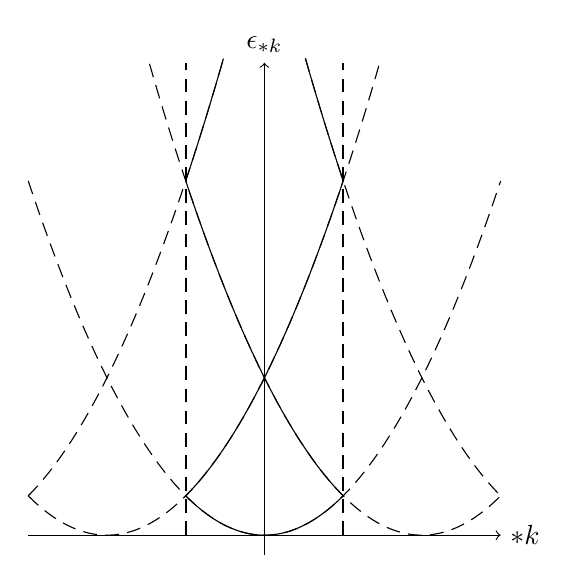
\begin{tikzpicture}
        
            % 动量横轴
            \draw[->] (-3,0) -- (3,0) node[right] {$\vb*{k}$};
            % 动能纵轴
            \draw[->] (0,-0.25) -- (0,6) node[above] {$\epsilon_{\vb*{k}}$};

            % 布里渊区边界
            \draw[dash pattern=on5pt off3pt, thick] (-1, 0) -- (-1, 6);
            \draw[dash pattern=on5pt off3pt, thick] (1, 0) -- (1, 6);
            
            % 画出布里渊区以外的能谱
            
            \draw[dash pattern=on5pt off3pt,samples=50, smooth, domain=-3:1.46] plot(\x,{0.5*((\x+2)*(\x+2))});
            \draw[dash pattern=on5pt off3pt,samples=50, smooth, domain=-3:3] plot(\x,{0.5*((\x)*(\x))});
            \draw[dash pattern=on5pt off3pt,samples=50, smooth, domain=-1.46:3] plot(\x,{0.5*((\x-2)*(\x-2))});
            \draw[dash pattern=on5pt off3pt,samples=50, smooth, domain=0.52:3] plot(\x,{0.5*((\x-4)*(\x-4))});
            \draw[dash pattern=on5pt off3pt,samples=50, smooth, domain=-3:-0.52] plot(\x,{0.5*((\x+4)*(\x+4))});

            % 画出布里渊区内部的$\epsilon_{\vb*{k}}$曲线,以及由于晶格周期性而导致的能谱平移
            \draw[samples=50, smooth, domain=-1:1] plot(\x,{0.5*(\x*\x)});
            \draw[samples=50, smooth, domain=-1:1] plot(\x,{0.5*((\x-2)*(\x-2))});
            \draw[samples=50, smooth, domain=-1:1] plot(\x,{0.5*((\x+2)*(\x+2))});
            \draw[samples=50, smooth, domain=0.52:1] plot(\x,{0.5*((\x-4)*(\x-4))});
            \draw[samples=50, smooth, domain=-1:-0.52] plot(\x,{0.5*((\x+4)*(\x+4))});
    
        \end{tikzpicture}
        
    }
    \subfigure[相互作用打开能隙,形成分离的能带]{
        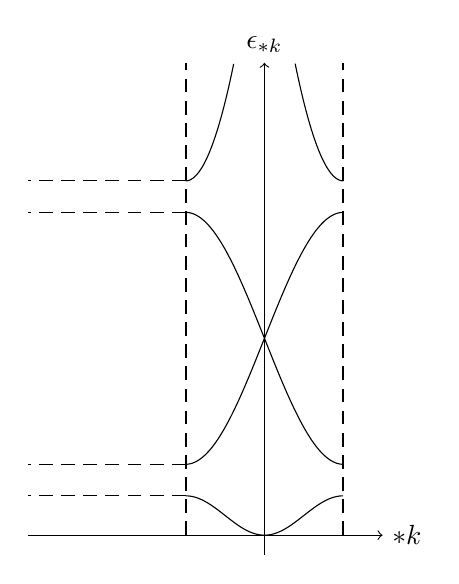
\begin{tikzpicture}
        
            % 动量横轴
            \draw[->] (-3,0) -- (1.5,0) node[right] {$\vb*{k}$};
            % 动能纵轴
            \draw[->] (0,-0.25) -- (0,6) node[above] {$\epsilon_{\vb*{k}}$};

            % 布里渊区边界
            \draw[dash pattern=on5pt off3pt, thick] (-1, 0) -- (-1, 6);
            \draw[dash pattern=on5pt off3pt, thick] (1, 0) -- (1, 6);
            
            % 画出布里渊区内部的$\epsilon_{\vb*{k}}$曲线,以及由于晶格周期性而导致的能谱平移
            \draw[samples=50, smooth, domain=-1:1] plot(\x,{0.25-0.25*cos(3.14*\x r)});
            \draw[samples=50, smooth, domain=-1:1] plot(\x,{2.5+1.6*sin(1.57*\x r)});
            \draw[samples=50, smooth, domain=-1:1] plot(\x,{2.5-1.6*sin(1.57*\x r)});
            \draw[samples=50, smooth, domain=0.39:1] plot(\x,{4.5+4*(\x-1)*(\x-1)});
            \draw[samples=50, smooth, domain=-1:-0.39] plot(\x,{4.5+4*(\x+1)*(\x+1)});

            % 标记能带和带隙
            \foreach \hei in {0.5, 0.9, 4.1, 4.5}
                \draw[dash pattern=on5pt off3pt] (-1,\hei) -- (-3, \hei);
    
        \end{tikzpicture}
        
    }
    \caption{能带结构}
    \label{fig:bloch-energy-band}
\end{figure}

两条不同的能带之间的间隙提供了一个自然的能量截断,因此在我们已经知道了系统的能带之后,如果需要一个低能有效理论,可以只考虑能量较低的能带,而将粒子跃迁到能量较高的能带再跃迁回来作为微扰,进行能量修正,即可以很自然地将高能能带积掉。

最后我们指定波函数的归一化方式。可以在积分号前面加上一个系数,即
\begin{equation}
    \frac{1}{V} \int \dd[3]{\vb*{r}} \psi_{n\vb*{k}}^*(\vb*{r}) \psi_{m\vb*{k}'}(\vb*{r}) = \delta_{mn} \delta(\vb*{k}-\vb*{k}'),
    \label{eq:bloch-is-basis}
\end{equation}
从而让简单的平面波$\exp(\ii \vb*{k} \cdot \vb*{r})$不需要乘上归一化因子就能够成为归一化本征态。
设$V_\text{u.c.}$是单个晶胞的大小,则
\[
    V = N V_\text{u.c.},
\]
从而可以得到
\begin{equation}
    \frac{1}{V_\text{u.c.}} \int_\text{u.c.} \dd[3]{\vb*{r}} u_{m\vb*{k}}^*(\vb*{r}) u_{n\vb*{k}}(\vb*{r}) = \delta_{mn}.
\end{equation}
只需要求解出一组满足以上条件的$\{u_{n\vb*{k}}\}$,就得到了一组正交归一化波函数$\{\psi_{n\vb*{k}}\}$。
归一化系数使用$V_\text{u.c.}$是非常合理的,因为如\eqref{eq:normalization-periodic}所示这正是具有正格子的周期性的函数通常使用的归一化系数。

\eqref{eq:bloch-is-basis}意味着布洛赫波函数是正交归一化波函数且对应的积分测度为
\[
    \frac{1}{\sqrt{V}} \int \dd[3]{\vb*{r}},
\]
记${c}_{n\vb*{k}}^\dagger$为位于能带$n$、格点动量为$\vb*{k}$的布洛赫电子的产生算符,那么%
\footnote{其中的$1/\sqrt{V}$的因子是因为二次量子化场算符通常使用全空间的积分为内积的定义,在此定义下,归一化的波函数是$\psi_{n\vb*{k}} / \sqrt{V}$而不是$\psi_{n\vb*{k}}$。}%
\begin{equation}
    {c}_{n \vb*{k}}^\dagger = \frac{1}{\sqrt{V}} \int \dd[3]{\vb*{r}} \psi_{n \vb*{k}}(\vb*{r}) {\psi}^\dagger(\vb*{r}),
\end{equation}
哈密顿量在这一组基下是对角化的,于是写出二次量子化哈密顿量(已经加入化学势项)
\begin{equation}
    {H} = \sum_{n, \vb*{k}} (\epsilon_{n\vb*{k}} - \mu) {c}^\dagger_{n\vb*{k}} {c}_{n\vb*{k}}.
    \label{eq:bloch-band-hamiltonian}
\end{equation}
$\vb*{k}$的取值局限在第一布里渊区内部,作为对比,不考虑周期势的边长为$L$的正方体势阱中的电子的$\vb*{k}$可以取遍所有位于那个边长为$2\pi / L$的格点。
但实际上两者的自由度是一样的,因为我们还有$n$标记各个能带,也即,我们相当于把所有能带中的动量都移动到了第一布里渊区内部。

\subsubsection{Wannier电子和紧束缚模型}

前面看到,我们使用了两个标签来标记一个电子模式:一个是“晶格动量”$\vb*{k}$,一个是能带编号。
前者的可能取值的数量有多少?晶格动量加上一个倒格矢之后与之前等价,因此晶格动量的取值数目为
\[
    \frac{2\pi / V}{2\pi / V_\text{u.c.}} = N,
\]
$N$为晶胞数目。当然这就是第一布里渊区中的动量数目。
一个晶格内可以有多种原子,但是这个信息已经被能带编号考虑在内了,因为电子“看到”原子种类的方式就是原子施加的势场,而周期势导致能带出现。
任何一种非布洛赫波函数的电子波函数基底也应该有同样的数目,例如,它们可以用一个“坐标”和一个能带编号标记。

本节讨论一种非常局域的电子基底。
一些时候,电子被强烈地束缚在原子周围,以至于除此之外的所有轨道都无需讨论。这种电子状态称为\concept{Wannier波函数}。
我们使用$i, j, \ldots$表示格点坐标,$m, n, \ldots$用于区分定域在$i$号晶胞附近的电子的电子云的形状(例如定域在某个格点附近的电子可以非常定域,也可以比较定域,有两种模式),$\vb*{r}_i$表示$i$处的格点的位矢,则定域在$i$号晶胞附近的Wannier电子的波函数可以用$w_{ni}(\vb*{r})$表示。
$i$的取值个数也是$N$,因此我们可以猜测,$i$与布洛赫电子的晶格动量对应,而$n$与能带编号对应。

定义在晶格格点上的函数以第一布里渊区为动量空间。
\[
    w_{ni}(\vb*{r}) \propto \sum_{\vb*{k}} \psi_{n\vb*{k}}(\vb*{r}) \ee^{- \ii \vb*{k} \cdot \vb*{r}_i},
\]
上式前面的归一化系数尚未选定。在归一化布洛赫波函数时我们使用了积分测度
\[
    \frac{1}{V} \int \dd[3]{\vb*{r}},
\]
从而导致归一化条件中出现了关于整块晶体的参数$V$。对布洛赫波函数这是合理的,因为它的好量子数是动量,因此是非常不定域的波函数,但Wannier波函数使用格点坐标标记,因此是非常定域的波包,因此我们希望Wannier波函数的归一化因子应该是一个常数而不包含任何关于系统大小的信息。
容易计算出
\[
    \frac{1}{V} \int \dd[3]{\vb*{r}} \frac{1}{N} \left( \sum_{\vb*{k}} \psi^*_{n\vb*{k}}(\vb*{r}) \ee^{\ii \vb*{k} \cdot \vb*{r}_i} \right) \left( \sum_{\vb*{k}} \psi_{m\vb*{k}}(\vb*{r}) \ee^{- \ii \vb*{k} \cdot \vb*{r}_j} \right) = \delta_{mn} \delta_{ij},
\]
取
\begin{equation}
    w_{ni}(\vb*{r}) = \frac{1}{N} \sum_{\vb*{k}} \psi_{n\vb*{k}}(\vb*{r}) \ee^{-\ii \vb*{k} \cdot \vb*{r}_i}, \quad \psi_{n\vb*{k}} = \sum_{\vb*{r}_i} \ee^{\ii \vb*{k} \cdot \vb*{r}_i} w_{ni}(\vb*{r}),
\end{equation}
这样归一化条件就是
\begin{equation}
    \frac{1}{V_\text{u.c.}} \int \dd[3]{\vb*{r}} \abs{w_{ni}(\vb*{r})}^2 = 1.
\end{equation}
归一化常数是一个局域的晶胞体积,符合我们的要求。

现在来分析Wannier波函数在实空间中的具体形状。考虑到$u_{n\vb*{k}}$的周期性,我们有
\[
    u_{n\vb*{k}} (\vb*{r}) = u_{n\vb*{k}} (\vb*{r} - \vb*{r}_i),
\]
于是
\begin{equation}
    w_{ni}(\vb*{r}) = \frac{1}{N} \sum_{\vb*{k}} u_{n\vb*{k}} (\vb*{r} - \vb*{r}_i) \ee^{\ii \vb*{k} (\vb*{r} - \vb*{r}_i)},
\end{equation}
这表明Wannier波函数实际上是$\vb*{r} - \vb*{r}_i$的函数,可以写成
\begin{equation}
    w_{ni}(\vb*{r}) = w_{n}(\vb*{r} - \vb*{r}_i),
\end{equation}
这当然是正确的,因为晶格中绝对位置$\vb*{r}$并无意义。
在$\vb*{r}$远离$\vb*{r}_i$时,指数因子快速振荡,导致整个求和基本上为零,因此Wannier函数只在$\vb*{r}_i$附加有较明显的值,因此它定域在格点$\vb*{r}_i$附近。

同样,Wannier波函数既然是一组正交归一化基底,就可以定义对应的二次量子化算符,即
\begin{equation}
    {c}^\dagger_{ni} = \frac{1}{\sqrt{V_\text{u.c.}}} \int \dd[3]{\vb*{r}} w_{ni}^*(\vb*{r}) {\psi}^\dagger(\vb*{r}).
\end{equation}

总之,晶格中的电子的波函数可以以高度定域在格点附近的一组波函数为基底,并且以对应的格点为一个量子数。

之前我们用\eqref{eq:bloch-band-hamiltonian}给出了布洛赫基下的能带理论哈密顿量。现在来看同样的理论在Wannier基下会呈现什么形式。
设能带理论下单电子哈密顿量为${h}$,则可以做表象变换
\[
    {H} = \sum_{mi, nj} {c}^\dagger_{mi} \mel{mi}{{h}}{nj} {c}_{nj},
\]
其中我们令
\begin{equation}
    - t_{mi, nj} = \mel{mi}{{h}}{nj} = \frac{1}{V_\text{u.c.}} \int \dd[3]{\vb*{r}} w_m^*(\vb*{r} - \vb*{r}_i + \vb*{r}_j) {h} w_n(\vb*{r}),
\end{equation}
则
\[
    {H} = - \sum_{mi, nj} t_{mi, nj} {c}^\dagger_{mi} {c}_{nj}.
\]
记号$\{mi, nj\}$表示对一组顺序不限的$\{mi, nj\}$组合只求和一次,就得到
\begin{equation}
    {H} = - \sum_{\{mi, nj\}} (t_{mi, nj} {c}_{mi}^\dagger {c}_{nj} + \text{h.c.}).
    \label{eq:hamiltonian-in-wannier}
\end{equation}
我们得到了一个非对角化的哈密顿量,这当然是正确的,因为系统显然应该在动量基——即布洛赫基——下对角化。
但\eqref{eq:hamiltonian-in-wannier}提供了非常清晰的物理图像:电子会从一个格点跃迁到另一个格点。
将电子的产生湮灭算符做傅里叶变换,立刻可以看出有能带产生。因此Wannier电子经过一个线性变换,也会变成能带电子。

最后考虑一个极限情况。假定晶格的吸引作用是如此之强,以至于电子是高度定域的,这样只有最近邻的格点之间才会跃迁。
进一步,考虑一个单能带的低能有效理论,就得到
\begin{equation}
    {H} = - \sum_{\pair{i, j}} (t_{ij} {c}^\dagger_i {c}_j + \text{h.c.}).
\end{equation}
这称为\concept{紧束缚模型}。如果满足平移不变性,就有
\begin{equation}
    {H} = - \sum_{\pair{i, j}} (t {c}^\dagger_i {c}_j + \text{h.c.}).
\end{equation}

本节只是从对称性的角度出发分析了哈密顿量的可能形式。哈密顿量的系数的具体计算需要专门的对电子能带结构的分析。

\subsubsection{声子}

实际上,离子实也会运动,于是我们得到一个定义在正格子上的场,这个场的激发就是\concept{声子}。晶体中一定会出现这样的激发,且这是一个Goldstone模式,因为晶体的形成实际上破缺了连续平移对称性,那么必然有一种零质量激发产生。
离子实的哈密顿量大致如下:(使用大写字母以和电子区分)
\begin{equation}
    {H} = \sum_n \frac{{P}_n^2}{2M_n} + \frac{1}{2} \sum_{\pair{m, n}} \omega_{mn}^2 ({X}_{m} - {X}_{n})^2 + \cdots, 
\end{equation}
其中$n$指的是晶格坐标,也就是三元组$(n_1, n_2, n_3)$,
\[
    \vb*{X} = \vb*{R} - \vb*{R}_0
\]
为某个离子实的位移。
正则量子化之后,哈密顿量中的前两项给出一个自由场,而离子实之间的非线性相互作用则给出声子-声子散射过程。
由于坐标-动量关系是对易关系而不是反对易关系,声子是玻色子。

离子实和电子的相互作用通常取这样的形式:
\[
    H_\text{ei} = \sum_{n, i} V_\text{ei}(\vb*{r}_i - \vb*{R}_n) = \sum_{n, i} (\vb*{R}_n - \vb*{R}_{n}^0) \cdot \grad{V_\text{ei}}(\vb*{R}_n^0 - \vb*{r}_i) + \cdots,
\]
其中$R^0_n$指的是离子实$n$未发生移动时的位置,即$n$号正格子的位置。
对位移场$\vb*{X}$做正则量子化,并将关于电子的部分做二次量子化,得到
\[
    {H}_{\text{ei}} = \sum_{n, i} V_\text{ei}(\vb*{r}_i - \vb*{R}_n) = \sum_{n} \int \dd[3]{\vb*{r}} {\vb*{X}} \cdot {\psi}^\dagger(\vb*{r}) \grad{V_\text{ei}}(\vb*{R}_n^0 - \vb*{r}) {\psi}(\vb*{r}) + \cdots,
\]
这就是电子-声子相互作用。可以看出以上哈密顿量对${\vb*{X}}$不具有$U(1)$对称性,因此声子一般来说不是守恒的。

声子和电子的量子化过程很不一样。对电子,我们首先写出一个多体一次量子化哈密顿量,然后做二次量子化;而对声子,我们实际上把使用格点坐标标记的离子实位移和动量当成了场算符(离散的场),然后直接对这两个场算符做正则量子化。
换而言之,没有声子的一次量子化:定义声子时我们的理论就是二次量子化的。

\subsubsection{自旋}

自旋是电子的内禀性质。然而,在一些情况下,电子几乎总是定域在某些格点附近而不发生移动,此时系统中不存在电子位置的变化,主要的自由度是各个格点上的自旋。
这样的模型即为所谓\concept{自旋模型}。自旋模型是非常常见的,如Hubbard模型在$U$非常大时,以动能项为微扰就能够得到一个海森堡模型。
对称性说明自旋-自旋相互作用通常可以取$\vb*{S}_i \cdot \vb*{S}_j$的形式,或者也许是各向异性的$\vb*{S}_i \cdot \vb*{T} \cdot \vb*{S}_j$。

\subsection{固体系统的宏观性质}

表征一个固体系统通常可以使用的方法,或者说固体系统常见的可测量量(这里不是指可观察量算符,而是指真的做量子测量能够测出来的物理量,比如说期望,等等),包括导电性、磁性、对电磁波的响应、力学和热学性质。

热学性质——从而固体力学性质——经常可以使用自由粒子的模型来估计。
一种无相互作用的粒子的哈密顿量是完全对角化的:
\[
    H = \sum_{\vb*{k}, \sigma} \omega_{\vb*{k}\sigma} \left(n_{\vb*{k} \sigma} + \frac{1}{2}\right),
\]
于是对配分函数的贡献为
\begin{equation}
    Z = \sum_{E_i} \ee^{- \beta E_i} = \ee^{-\beta E_{\text{eq}}} \prod_{\vb*{k}, \sigma} \ee^{- \beta \frac{\omega_{\vb*{k}\sigma}}{2}} \sum_{n_{\vb*{k}, \sigma}} \ee^{-\beta \omega_{\vb*{k}\sigma} n_{\vb*{k} \sigma}},
\end{equation}
因此这种粒子对内能的贡献为
\begin{equation}
    U = E_{\text{eq}} + \sum_{\vb*{k}, \sigma} \left( \frac{1}{2} + \frac{1}{\ee^{\beta \omega_{\vb*{k}\sigma}} - 1} \right) \omega_{\vb*{k}\sigma}.
\end{equation}
这样,等容热容为
\begin{equation}
    C_V = \left(\pdv{U}{V}\right)_V = \sum_{\vb*{k}, \sigma} \left(\frac{\omega_{\vb*{k}\sigma}}{T}\right)^2 \frac{\ee^{\omega_{\vb*{k}\sigma} / T}}{(\ee^{\omega_{\vb*{k}\sigma} / T} - 1)^2}.
\end{equation}
每种粒子都会对热容有一个贡献,相互作用会修正这个贡献。

如果一种粒子携带某种荷,那么还可以观察到\concept{输运}。大体上输运过程可以分成两种,一种是粒子平均自由程远小于系统尺寸的过程,此时系统内部足以出现荷的梯度,输运流量和这种梯度有关,可以称为\concept{扩散};另一种是粒子平均自由程大于系统尺寸的过程,此时系统内部的粒子基本上不受到任何阻碍,输运流量由系统边界上的性质确定,即所谓\concept{弹道输运}。
